% LTeX: language=spanish

% TODO

% Quitar los títulos de la introducción; que se queden como ideas principales.
% Mencionar sistemas de clim. en la introducción brevemente. Buscar ejemplos concretos para cada uno.
% Ampliar soluciones corporativas. Bastante.
% Referencias.
% En general se ha centrado bastante a la introducción.
% Utilizar el concepto de Green IT
% Añadir citas en las imagenes

\chapter{Introducción}

Con la transición a la computación en la nube surge la necesidad de crear sistemas para suplir los requisitos de usuarios y organizaciones. Los \textbf{centros de procesamientos de datos} (CPD; en inglés, \textit{data centers}) son los lugares donde se instala el equipamiento necesario para conseguir este objetivo.

Un centro de datos está compuesto por componentes informáticos como routers, switches, firewalls, sistemas de almacenamiento masivo de datos y sistemas de cómputo. Para que funcionen a pleno rendimiento, es esencial saber cómo organizar estos sistemas; tanto informática como físicamente. A fin de cuentas, es inevitable tener que combatir el archienemigo de la electricidad: \textbf{el calor}.

Cualquier dispositivo tecnológico está condenado a producir calor para operar. Esto es inevitable. Si tenemos en en cuenta la concentración de equipamiento que se produce en un CPD, disipar el calor producido por todos se vuelve un problema serio. Si no se refrigeraran, su vida útil se acortaría, la capacidad de cómputo se vería mermada debido al \textit{thermal throttling} de las CPUs modernas, el \textit{downtime} aumentaría significativamente... Además, las consecuencias medioambientales serían desastrosas. Por todo estos motivos, debemos buscar métodos de transferencia de calor.


En este trabajo abordaremos la última parte. En particular, estudiaremos las diferentes \textbf{técnicas de refrigeración} de un centro de datos, comparando las diferentes soluciones.

\section{¿Por qué es importante la refrigeración?}


Se estima que, en 2020, el consumo de los centros de datos supuso un 1 - 1.5\% de la producción de electricidad global \cite{mytton-dc}. Con la llegada de la pandemia y la transición al trabajo remoto, esta cifra ha debido aumentar en los últimos dos años; y la tendencia sigue en aumento. Aunque las arquitecturas modernas necesitan menos energía para operar con un uso bajo, el consumo medio de un rack es de 7 kW, llegando a picos de incluso 20 kW por rack \cite{datacenters-density}.

El sistema de refrigeración puede suponer hasta un 40\% del consumo energético del CPD. Una parte importante de este 40\% la componen los ventiladores (12\% del total) y los enfriadores del agua (14\% del total) \cite{ZHANG2021102253}

\begin{figure}
    \begin{center}
    \caption{Consumo energético del CPD.}
    \label{consumo_energetico}
    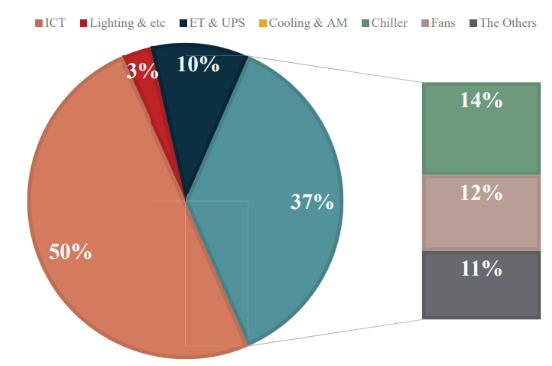
\includegraphics[scale=1]{consumo}
    \end{center}
\end{figure}

\section{Cómo funciona un sistema de refrigeración}

Aunque, como veremos más adelante, existen diferentes técnicas de refrigeración, todas tienen como objetivo principal \textbf{reducir la temperatura de un equipo}. Debido al poco espacio disponible en un sistema, todos los métodos usarán algún medio para transferir el calor a otro lugar. Esta es una forma muy eficiente de refrigerar un sistema, pues resulta más sencillo mover todo el calor a otra parte para tratarlo en un lugar específico, en lugar de trabajar equipo a equipo. Esta es la misma base que se utiliza en los ordenadores personales, aunque a una escala mucho mayor.

En general, un sistema de climatización tendrá los siguientes componentes:

\begin{itemize}
    \item Un generador del medio a utilizar para transferir el calor.
    \item Una vía por la que viaja el medio. Pueden ser cables, el aire, un pasillo...
    \item Una fase de transferencia de calor del sistema o habitación al medio.
    \item Una forma mediante la cual se enfría el medio.
\end{itemize}

La escala del sistema de refrigeración dependerá de cómo de ambicioso sea el centro de datos. Teniendo en cuenta la \textit{tier} del CPD \cite{cofrico}, se usará un tipo u otro; dependiendo de la robustez que aporten.

\chapter{Preliminares}

\chapter{Desarrollo}

\section{Sistemas de climatización}

Para climatizar los centros de datos, existen tres vías principales:

\begin{itemize}
    \item \textbf{A través del aire}. Se basan en conductos de aire para enfriar los diferentes dispositivos. Estos conductos bombean aire frío hacia los equipamientos y luego recogen el aire caliente que sale de estos. De esta forma, se consigue separar el aire caliente del frío. Un importante inconveniente es que este tipo de sistemas requiere un gran consumo de energía.
    \item \textbf{A través del agua}. Se basan en grandes contenedores de agua fría. El funcionamiento de este tipo de sistemas consiste en bombear el agua a través de las tuberías que pasan entre los dispositivos y los racks. Es importante mantener siempre una barrera entre los dispositivos y el agua que circula, pues si se produce contacto entre ellos se podrían dañar los componentes.
    \item \textbf{Inmersión}. Se basan en la inmersión de los equipos de IT en un fluido dieléctrico que no conduce la electricidad pero si es capaz de llevarse el calor de los chips de los equipos. Este tipo de sistemas destaca por ser el más eficiente sin necesidad de necesitar sistemas de refrigeración con gases fluorados.
\end{itemize}

\section{Técnicas de refrigeración}

\subsection{Aire}

En este apartado estudiaremos las distintas técnicas cuya vía principal para climatizar los CPD es el aire.

\subsubsection{Free cooling}

Free cooling es una técnica efectiva para asegurar que el flujo de temperatura de un centro de procesamiento de datos está funcionando adecuadamente. Esta técnica requiere de un coste mínimo, por lo que reduce los gastos totales de la refrigeración del CPD.

Este método consiste en dos sistemas, uno de economización de aire y otro de economización de agua. La economización de aire usa el aire del exterior del centro de procesamiento de datos para regular la temperatura de los equipos del interior del CPD, dejándolo entrar a este. Mientras que la economización de agua % TODO

% TODO: explicar el sistema de economización de agua

Generalmente, con el fin de evitar que entre humedad o partículas contaminantes se suele realizar un filtrado del aire.

En la imagen \ref{free_coling} podemos observar un esquema del funcionamiento de esta técnica.

\begin{figure}
    \begin{center}
    \caption{Esquema del free cooling.}
    \label{free_coling}
    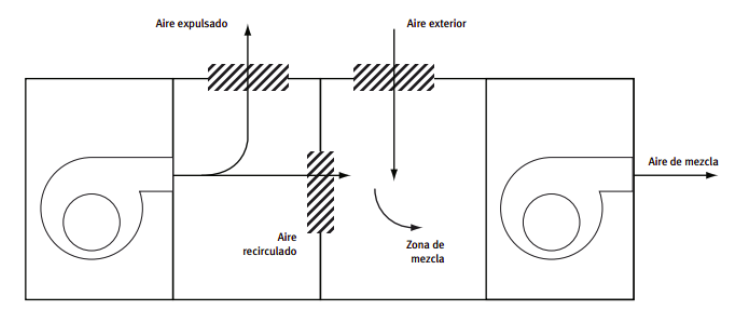
\includegraphics[scale=1]{free_cooling}
    \end{center}
\end{figure}

Esta técnica tiene varias ventajas, pues permite ahorrar y mejora la calidad del aire interior. Sin embargo, requiere de un mínimo consumo y de un mecanismo complejo de ventiladores, compuertas y filtros.

\subsubsection{Pasillos calientes y fríos}

Esta técnica tiene como objetivo separar por completo el aire frío proveniente del aire acondicionado y el aire caliente que expulsan los equipos. Para ello, se aprovecha el diseño de los racks de servidores y la disposición de los mismos en el centro de procesamiento de datos. Esto es, se alinean los racks en filas alternas (frío/caliente), dejando todas las entradas de aire frío hacia un lado y las salidas de aire caliente hacia el otro. Así, las filas compuestas por frentes de racks se llaman pasillos fríos, que suelen enfrentar a los conductos de salida del aire acondicionado, y la parte trasera de los racks, por donde se expulsa el aire caliente, se denominan pasillos calientes, que suelen conectarse a los conductos de retorno del aire acondicionado.

En las imágenes \ref{pasillos} y \ref{traditional_cooling} podemos observar unos esquemas del funcionamiento de esta técnica.

\begin{figure}
    \begin{center}
    \caption{Esquema de los pasillos calientes y fríos.}
    \label{pasillos}
    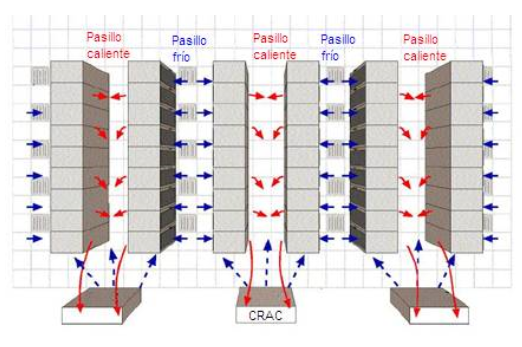
\includegraphics[scale=1]{pasillos}
    \end{center}
\end{figure}

Esta técnica suele combinarse con el método de falsos suelos y techos para facilitar el paso del aire.

Además, mediante esta técnica se conserva la energía y se reducen los costes de enfriamiento por la gestión del flujo de aire.

\begin{figure}
    \begin{center}
    \caption{Diagrama de enfriamiento tradicional.}
    \label{traditional_cooling}
    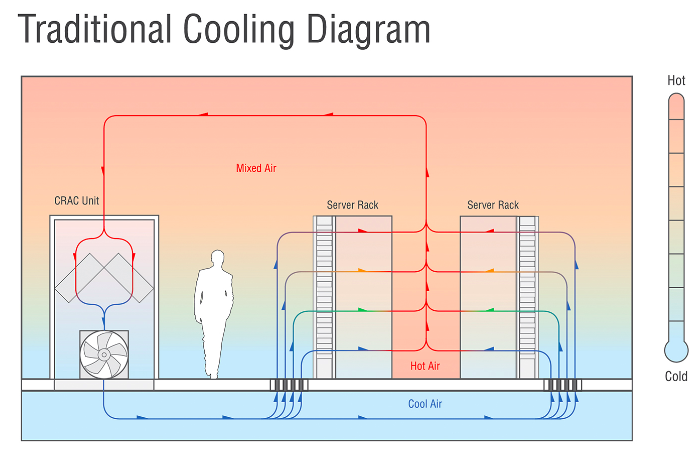
\includegraphics[scale=1]{traditional_cooling_diagram}
    \end{center}
\end{figure}

\subsubsection{Confinamiento de zonas}

Esta técnica se basa en aislar los pasillos fríos de los calientes mediante la colocación de cerramientos. De esta forma, los pasillos podrán recibir la circulación de los flujos de aire correspondiente sin que se produzca una mezcla de corrientes sin control.

En la imagen \ref{hot_aisle} podemos observar un esquema del funcionamiento de esta técnica.

\begin{figure}
    \begin{center}
    \caption{Diagrama de cerramiento de pasillo caliente.}
    \label{hot_aisle}
    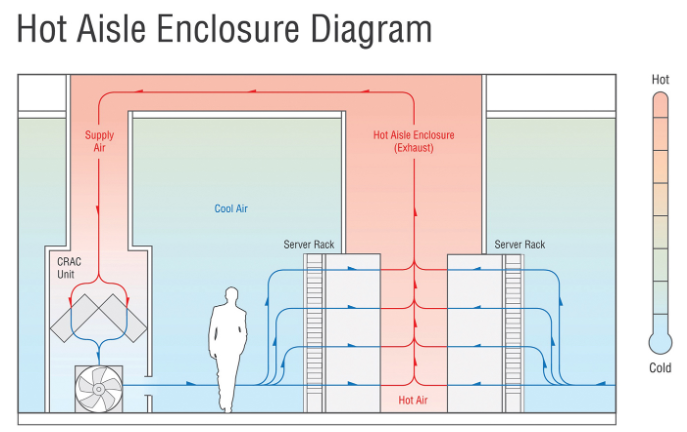
\includegraphics[scale=1]{hot_aisle}
    \end{center}
\end{figure}

\subsubsection{Refrigeración adiabática}

Esta técnica es capaz de utilizar la baja humedad relativa del aire para incorporar agua y evaporarla, por lo que consigue lograr una importante reducción de temperatura. Una ventaja es que no necesita un importante consumo energético.

En la imagen \ref{adiabatic_coolers} se muestra un 
\begin{figure}
    \begin{center}
    \caption{Enfriamientos adiabáticos}
    \label{adiabatic_coolers}
    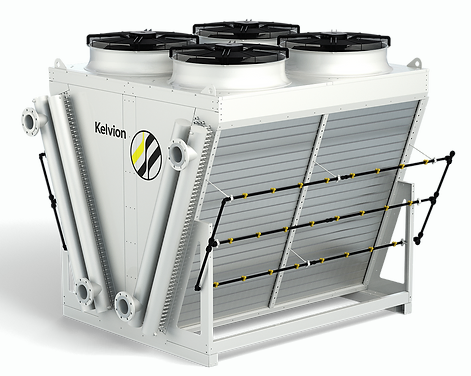
\includegraphics[scale=1]{adiabatic_coolers}
    \end{center}
\end{figure}

\subsubsection{In-Rack Heat Extraction}

La idea de este método de refrigeración se basa en extraer el calor que se genera dentro del rack para que ni siquiera entre en la sala de servidores.

\subsubsection{Aire acondicionado para la sala de ordenadores (CRAC)}

Las unidades CRAC son similares a equipos usuales de aire acondicionado que funcionan gracias a un compresor, el cual atrae aire a través de una unidad cargada con refrigerante. De esta manera, se introduce el aire frío en el centro de procesamiento de datos.

Son bastante comunes en muchos centros de datos, ya que a pesar de su alto consumo de energía, el coste del equipo es muy bajo.

\subsubsection{Controlador de aire para la sala de ordenadores (CRAH)}

Una unidad CRAH funciona dentro de un sistema más amplio que involucra una planta de agua enfriada. Este agua fluye a través de un conducto de enfriamiento dentro de la unidad, que luego usa ventiladores de modulación para extraer aire del exterior de la instalación. Estas unidades serán más eficientes si se usan en lugares con temperaturas más frías, pues tendrán que enfriar menos el aire exterior.

\subsubsection{Refrigeración vectorial calibrada (CVC)}

Esta tecnología de enfriamiento está hecha específicamente para servidores de alta densidad. Optimiza la ruta del flujo de aire a través del equipo para permitir que el sistema de enfriamiento maneje el calor de manera más efectiva, lo que hace posible aumentar la proporción de placas de circuito por chasis de servidor y utilizar menos "enthusiasts" (\textcolor{red}{no sé cómo se traduce enthusiasts aquí}).

\subsubsection{Falsos suelos y techos}

Los suelos y techos técnicos para centros de datos son suelos y techos que pueden instalarse a distintas alturas, dejando un hueco entre esta instalación y los suelos y techos "reales".

Es usual que los suelos consistan en rejillas de ventilación, pues son convenientes para servicios de refrigeración, eléctricos y mecánicos. De esta forma, con menos gasto de energía se puede ayudar en la refrigeración de los servidores, por ejemplo centrando las salidas de aire bajo las máquinas.

También resulta útil para facilitar el acceso al cableado. En este aspecto, el falso techo supone más problemas que el suelo, pues requiere usar guías y escaleras para acceder a él, pero con el falso suelo solo hay que levantar las baldosas y realizar los ajustes necesarios.

Por último, cabe destacar que estos suelos dan flexibilidad, pues pueden instalarse a la altura que se requiera y pueden reutilizarse si se reformara el CPD o se cambiara la localización del mismo.

\subsubsection{Expansión directa (DX cooling)}

Esta técnica utiliza los principios de la termodinámica para transferir calor de un área a otra a través de la evaporación y condensación de un refrigerante, que sirve como medio a través del cual el calor se captura y se elimina de un área y se libera en otra. Por ejemplo, los aires acondicionados usan este mecanismo para mover el calor de una habitación hacia el exterior.

Este sistema tiene las siguientes componentes:

\begin{itemize}
    \item {\textbf{El refrigerante}}, que es el medio que fluye a través del sistema, recolectando y disipando el calor en diferentes áreas.
    \item \textbf{El compresor}, que es una carga de motor eléctrico y suministra la energía para impulsar el refrigerante a través del sistema.
    \item \textbf{El evaporador}, que recoge el calor del recinto y facilita la ebullición del refrigerante.
    \item \textbf{El condensador}, que disipa el calor en el medio ambiente al permitir que el refrigerante vuelva a su estado líquido.
    \item \textbf{La válvula de expansión}, que actúa como regulador entre el lado de alta y baja presión del sistema y permite la caída de presión y temperatura necesaria para facilitar la expansión directa.
\end{itemize}

\subsection{Agua}

En este apartado estudiaremos las distintas técnicas cuya vía principal para climatizar los CDP es el agua.

\subsubsection{Sistema de agua helada}

Este método se usa comúnmente en centros de datos de tamaño mediano a grande que usan agua caliente para enfriar el aire que producen los controladores de aire (CRAH). Para ello, se usa una planta enfriadora para suministrar el agua.

\subsubsection{Enfriamiento evaporativo}

Esta técnica expone el aire caliente al agua, lo que produce la evaporación del agua y así extraer el calor del aire. Este sistema es extremadamente eficiente desde el punto de vista energético, sin embargo utilizará mucha agua.

\subsection{Inmersión}

En este apartado estudiaremos las distintas técnicas cuya vía principal para climatizar los CDP es la inmersión.

\subsubsection{Refrigeración por inmersión}

En este método, el hardware se sumerge en un fluido dieléctrico no conductor e inflamable (\textcolor{red}{non-flammable era inflamable o flamable?}) \textcolor{red}{INFLAMABLE SIGNIFICA FLAMABLE}?, introduciendo tanto el líquido como el hardware en un contenedor a prueba de fugas. De esta manera, el líquido absorbe el calor mientras que el agua caliente se convierte en vapor, para luego condensarse al enfriarse y vuelve al líquido refrigerante, ayudando así a que este se enfríe de nuevo.

Cabe destacar que esta técnica es muy eficaz, pues el fluido absorbe el calor mucho más eficientemente que el aire.

\section{Soluciones corporativas}

% TODO: ampliar

En esta sección presentaremos algunas empresas que se dedican a suministrar los productos necesarios para conseguir soluciones de refrigeración para centros de datos.

Un ejemplo es la empresa Systemair, que ofrece una gran variedad de productos en este catálogo para asegurar sistemas de refrigeración energéticamente eficientes, tales como unidades de enfriamiento gratuito, sistemas de enfriamiento evaporativo compacto con pre enfriamiento del aire exterior, condensadores para la expansión directa, etc.

Otra alternativa es Clysema, una empresa de servicios energéticos enfocada a mejorar la eficiencia energética de las instalaciones. Ofrecen servicios de gestión y optimización, auditoría, ejecución y mantenimiento.

Otras empresas que están ayudando a innovar la industria de los centros de datos son LiquidStack, Submer, Asperitas, Usystems, Munters, Green Revolution Cooling, STULZ, etc.



\section{Futuro}

Desde hace varios años, los centros de procesamiento de datos han incrementado su potencia y número de servidores significativamente, lo que implica la necesidad de encontrar métodos de enfriamiento más eficaces y mejores para poder enfriar estos centros de datos.

Por tanto, actualmente se están investigando nuevas técnicas de enfriamiento que se espera que puedan ponerse en práctica lo antes posible. Principalmente se está trabajando sobre técnicas con refrigeración líquida, ya que son mucho más efectivas, pues los fluidos absorben mejor el calor que el aire.

\subsection{Tecnologías de refrigeración líquida}

A diferencia del enfriamiento por aire, que requiere mucha energía e introduce contaminantes y condensación en el centro de datos, un sistema de enfriamiento líquido es más limpio, más escalable y altamente específico. Actualmente, se están desarrollando dos métodos: enfriamiento por inmersión total y enfriamiento directo del chip.

\subsubsection{Refrigeración directa del chip}

La refrigeración directa del chip usa tuberías que transportan el líquido refrigerante directamente a una placa fría que se sitúa encima de los chips de una placa base para extraer el calor. El calor extraído se lleva a un circuito de agua enfriada para ser transportado de nuevo a la planta de enfriamiento de la instalación  y expulsado al exterior.

Este método proporciona una forma muy eficaz de enfriamiento para centros de datos que usan mucha potencia y, por tanto, necesitan métodos muy potentes de enfriamiento.

\chapter{Conclusiones}

% TODO

%Bibliografía
%Data Center Cooling: Future of Cooling Systems, Methods and Technologies (datacenters.com)

%Data Center Cooling 101: A Beginner's Guide to AFM Best Practices and Cooling Optimization - YouTube

%https://clysema.com/tendencias-climatizacion-centros-de-datos/

%https://www.systemair.com/fileadmin/user_upload/systemair-b2b/Local/Turkey/Destek/Medya_Merkezi/Veri_Merkezleri/Systemair-DataCentre-Cooling-Solutions_web.pdf

%https://www.rittaltic.es/importancia-refrigeracion-centros-datos/

%https://journal.uptimeinstitute.com/a-look-at-data-center-cooling-technologies/

%Datacenter Cooling Methods | Datacenter cooling best practices (submer.com)

%Types of Data Center Cooling Techniques - Raritan

%https://www.siberzone.es/blog-sistemas-ventilacion/enfriamiento-adiabatico/

%(152) What Is A Quick-Connect Fitting And How Do They Work? - YouTube

%https://opentextbc.ca/basichvac/chapter/direct-expansion-air-conditioning-systems/

%https://www.airzone.es/blog/ahorro/que-es-el-free-cooling/

%https://blog.logisa.com/blog/diferencia-entre-contencion-de-pasillos-frios-y-de-pasillos-calientes

%Data center - Wikiwand

%What Is a Data Center? - Cisco

%[1] How much energy do data centers use? David Mytton (no sé cómo poner referencias aquí, luego lo vemos)

%[2] The Rising Data Center Power Density and The Resultant Challenges (datacenters.com)

%[3] A survey on data center cooling systems: Technology, power consumption modeling and control strategy optimization - ScienceDirect

%[4] La importancia de la Refrigeración de los Centros de Datos (cofrico.com)

%Choosing the right PC cooling system for you | reichelt.com|Choosing the right PC cooling system for you | reichelt.com

%https://pavimentostecnicos.com/suelo-tecnico/falso-suelo-para-cpd
